\documentclass{article}
\usepackage[letterpaper, margin=2cm]{geometry}
\usepackage[utf8]{inputenc}
\usepackage{amssymb}
\usepackage{amsmath}
\usepackage{bm}

\usepackage{subfig}

\setlength\parindent{0pt}

\usepackage{graphicx}
\graphicspath{{../figures/}}

\usepackage{soul}

\DeclareMathOperator*{\argmin}{arg\,min}
\DeclareMathOperator*{\argmax}{arg\,max}

\title{A dissimilitude-based constructive algorithm for a maximum profit facility location problem on the metric-space}

\author{Francisco J. A. Casas \and Renato F. J. Casas \and Claudio E. Torres}

\begin{document}

\maketitle

% TODO: Conocer hasta qué tamaños son capaces de tratar los métodos "eficientes en la práctica". Esto refuerza la necesidad de intentar resolver el modelo con programación dinámica...
\abstract{En el área del \emph{location analysis} los problemas de \emph{facility location} tratan de elegir la ubicación correcta de instalaciones para alcanzar un conjunto de clientes o puntos de demanda. Aunque la mayoría de estos problemas se caracterizan por su NP-completitud se han desarrollado métodos eficientes en la práctica para los más comunes, sin embargo los modelos determinados por la ganancia económica, donde entra en juego el costo de las instalaciones, transporte y la ganancia al alcanzar un cierto cliente, y la cantidad de instalaciones es endógena al problema, han recibido poca atención pese a estar más cerca del uso práctico de la ciencia, probablemente debido a que la posibilidad de elegir si cubrir o no cada cliente aumenta el costo computacional en la práctica. En este trabajo se introduce un modelo que representa estas características y se presenta un método constructivo basado en reducir en cada paso las soluciones encontradas a una población representativa utilizando una métrica de disimilitud espacial entre estas, pudiendo adaptarse los parámetros según la capacidad computacional disponible. Esta idea aprovecha que se esté trabajando sobre un espacio métrico en que la distancia determina los costos de transporte, lo que hace decaer de manera gradual la ganancia de agregar cada cliente, haciendo que la similitud geográfica de las soluciones está estrechamente relacionada con el potencial económico. Finalmente se discuten los resultados obtenidos para casos de prueba, comparando con un algoritmo voraz y con la solución óptima cuando es factible calcularla.
}
% NOTE: ¿Agregar una comparación con su formulación en programación lineal?

\section{Estado del Arte}

% TODO: Completar con el libro

% De acuerdo con la clasificación mencionada en \cite{revelle2005location},

En el área de la \emph{facility location} entre los problemas más comunes se tienen los modelos de cobertura, que intentan encontrar la cantidad mínima de instalaciones para alcanzar todos los clientes, los \emph{$p$-median} que minimizan la suma de las distancias a cada cliente y los \emph{center problems} que minimizan la mayor distancia de un cliente a una instalación, en ambos últimos la cantidad de instalaciones es un parámetro fijado a priori, pero en todos se tiene la necesidad de cubrir a todos los clientes \cite{owen1998strategic}, esta restricción \emph{serve all comers} es justificable en el sector público, pero en el sector privado se puede optar por no alcanzar un cliente lejano si el hacerlo aporta negativamente a las utilidades.

\cite{mukundan1991joint} muestra un modelo de maximización de utilidades, considerando costos de transporte y niveles de inversión para cada instalación (que permiten abarcar diferentes distancias), entre las variantes se propone  eliminar la restricción \emph{serve all comers}. \cite{brimberg2000maximum} muestra modelos bi-critero entre las ganancias o costos operativos y la inversión necesaria, entre otras cosas, para la compra y puesta en marcha de las instalaciones, al igual que el anterior realiza pruebas con solvers de programación lineal. Ambos trabajos concluyen que la relajación LP de los modelos sobre los que se hicieron pruebas son \emph{integer-friendly} pero no eliminan la restricción \emph{serve all comers} en estas pruebas, aun así  \cite{brimberg2000maximum} concluye que el aumentar el tamaño del problema deteriora la \emph{integer-friendliness}.

\section{Modelo}

% TODO: Agregar sobre la clasificación del problema (lo hago en la introducción ¿Borrar?)

% TODO: Señalar que aunque se habla de clientes pueden ser suministros, ¿Señalar aplicación en ubicación de plantas de biogas de papá?

Se tiene un conjunto de posibles ubicaciones para instalaciones $Z = \{z_1,z_2,...,z_{|Z|}\}$ y un conjunto ubicaciones de clientes $C = \{c_1,c_2,...,c_{|C|}\}$, cada cliente $c_i$ tiene asociado un peso o cantidad de demanda $w_i$.

Estas ubicaciones pueden ser vectores en $\mathbb{R}^N$, posiciones en una red o cualquier espacio métrico $\mathbb{E}$ en que se encuentre definida una métrica de distancia $d : \mathbb{E}^2 \rightarrow \mathbb{R}$ entre cada par de estas.

Se tiene el siguiente modelo de programación lineal:

\textbf{Índices:}
\begin{align*}
    i &= \text{índices de posibles clientes} \\
    j &= \text{índices de posibles ubicaciones de instalaciones} \\
    \text{\textbf{Inputs:}} \\
    w_i &= \text{Demanda del cliente $i$} \\
    \gamma &= \text{Costo fijo de colocar cada instalación} \\
    \alpha &= \text{Ganancia obtenida por cada unidad de demanda alcanzada} \\
    \beta &= \text{Costo de transportar una unidad de distancia una unidad de demanda} \\
    d_{ij} &= \text{Distancia entre cliente $i$ y la instalación $j$} = d(c_i,z_j)
\end{align*}

\textbf{Variables de decisión:}
\begin{align*}
    Y_{ij} &= \begin{cases}
        1 & \text{Si la demanda de $c_i$ es suplida por la instalación en $z_j$} \\
        0 & \text{Si no}
    \end{cases} \\
    X_{j} &= \begin{cases}
        1 & \text{Si se decide poner una instalación en $z_j$} \\
        0 & \text{Si no}
    \end{cases}
\end{align*}

\textbf{Maximizar:}
\begin{equation}
    - \sum_{j=1}^{|Z|} \gamma X_{j} + \sum_{i=1}^{|C|} \sum_{j=1}^{|Z|} \alpha w_i Y_{ij} - \sum_{i=1}^{|C|} \sum_{j=1}^{|Z|} \beta w_i d_{ij} Y_{ij}
\end{equation}

\textbf{Sujeto a:}
\begin{align*}
    Y_{ij} \leq X_{j} &\qquad \forall i \in \{1..|C|\} \quad \forall j \in \{1..|Z|\} \\
    \sum_{j=1}^{|Z|} Y_{ij} \leq 1 &\qquad \forall i \in \{1..|C|\} \\
    Y_{ij} = 0,1 &\qquad \forall i \in \{1..|C|\} \quad \forall j \in \{1..|Z|\} \\
    X_{j} = 0,1 &\qquad \forall j \in \{1..|Z|\}
\end{align*}

Este modelo corresponde a un caso particular de una de las variaciones mencionadas en \cite{mukundan1991joint}, en que los parámetros $d_{ij}$ cumplen con las propiedades de un espacio métrico, el costo de ubicar una instalación y la ganancia por alcanzar un cliente es independiente de su posición y el costo de transporte sólo depende de su nivel de demanda y su distancia.

\begin{figure}%
    \centering
    \subfloat[Ejemplo de un problema]{{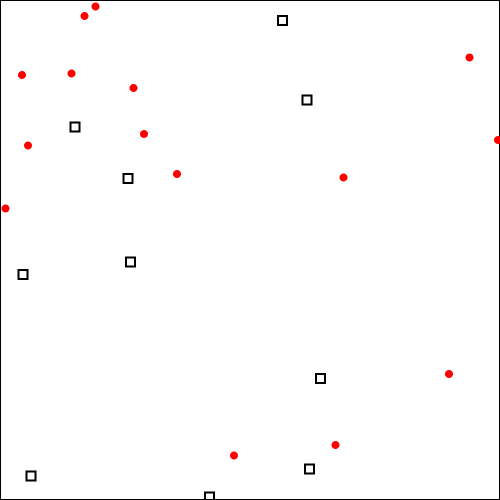
\includegraphics[width=5cm,height=5cm]{small_case_raw.png}}}
    \qquad \qquad \qquad
    \subfloat[Posible solución]{{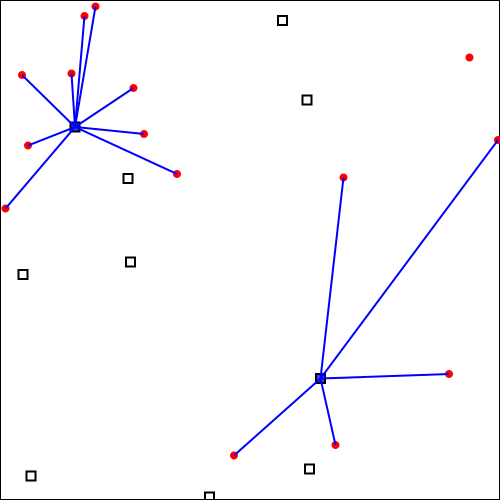
\includegraphics[width=5cm,height=5cm]{small_case_sol.png}}}
    \caption{A la izquierda, ejemplo de un problema, puntos rojos son ubicaciones de clientes, cuadrados son posibles ubicaciones de instalaciones.\\ A la derecha una posible solución, cuadrados azules representan subconjunto elegido de ubicaciones de instalaciones, clientes son trabajados por la instalación más cercana o ninguna si todas están muy lejos (tal es el caso del cliente en la esquina superior derecha).}
    \label{fig:problem}
\end{figure}

Notando que la función objetivo puede expresarse de la siguiente manera:
\begin{align*}
    -\sum_{j=1}^{|Z|} \gamma X_{j} + \sum_{i=1}^{|C|} w_i \sum_{j=1}^{|Z|} Y_{ij} (\alpha - \beta d_{ij})
\end{align*}

Es posible identificar un radio crítico $RC = \frac{\alpha}{\beta d_{ij}}$ pasado el cual no es conveniente suplir la demanda de un cliente. De la misma manera, puesto que la única variable controlable es $d_{ij}$, convendrá que la demanda de cliente sea suplida por la instalación colocada más cercana, a menos que esta se encuentre a una distancia mayor que el radio crítico.

La última observación permite expresar una solución al problema ya no como el conjunto de varibles de decisión $X_{j}$ y $Y_{ij}$, sino como un subconjunto $S$ de $Z$, buscando maximiziar el valor de la siguiente función objetivo $\Phi : \mathcal{P}(Z) \rightarrow \mathbb{R}$:

\begin{equation}
\Phi(S) = -\gamma \cdot |S| + \sum_{i=1}^{|C|} \max \left\{ 0 , \max_{z \in S} ( \alpha \cdot w_i - \beta \cdot w_i \cdot d(c_i,z)) \right\}
\end{equation}

Una solución $S$ se traduce a una solución para el modelo de programación lineal, asumiendo por simplicidad y sin pérdida de generalidad que las distancias $d_{ij}$ son diferentes, de la siguiente manera:

\begin{align*}
    X_{j} &= \begin{cases}
        1 &\quad z_j \in S \\
        0 &\quad z_j \notin S
    \end{cases}\\
    Y_{ij} &= \begin{cases}
        1 &\quad (d_{ij} \leq RC) \wedge (d_{ij} \leq d_{ik} \quad \forall k : z_k \in S)
        \\
        0 &\quad e.o.c.
    \end{cases}
\end{align*}

Siendo las soluciones generadas de esta manera siempre igual o mejores que sus contrapartes con distintos valores $Y_{ij}$, se reduce el espacio de búsqueda, a uno con soluciones descritas completamente por un subconjunto de instalaciones elegido.

% TODO: U N D E R S T A N D
% Una propiedad que vale la pena destacar es que si se tiene una solución $P$ y una instalación $q$:
% \begin{equation}
%     \Phi(P) > \Phi(P \cup \{q\}) \wedge (P \subseteq R) \RightArrow  \Phi(R) > \Phi(R \cup \{q\})
% \end{equation}

\section{Algoritmo}

El algoritmo comienza encontrando todas las ubicaciones de instalaciones que, por si solas, tienen función objetivo positiva:
\begin{equation}
G = \{ s |  \quad s \in Z, \quad \Phi(\{s\}) \geq 0 \}
\end{equation}
Estas ubicaciones forman la \emph{base} de soluciones de tamaño 1:
\begin{equation}
B_1 = \{ \{g\} | \quad g \in G \}
\end{equation}

El algoritmo procede realizando iteraciones, cada una consiste en un proceso de \textbf{reducción} de la base a una cantidad manejable de soluciones representativas (llámese \emph{pool}) y una posterior \textbf{expansión} de esta \emph{pool} para formar la \emph{base} de soluciones de tamaño mayor.

El proceso de reducción se puede escribir como:
\begin{equation}
P_n = Reduce(B_n)
\end{equation}
donde la función $Reduce$ se explicará más adelante. El algoritmo trabaja con un parámetro \texttt{POOL\_SIZE} que indica la cantidad máxima de soluciones que puede tener una \emph{pool}, una mayor \emph{pool} explorará más posibles soluciones pero tendrá un costo computacional mayor.

Por otro lado el proceso de expansión está dado por:
\begin{equation}
B_{n+1} = \{S = p \cup \{g\} |
    \quad p \in P_n, \quad g \in G, g \notin P_n, \forall (p \in P_n)( p \not\subset S \vee \Phi(p) < \Phi(S)) \}
\end{equation}
Este consiste en tomar cada solución de la \emph{pool} y agregarle una nueva instalación de $G$ de todas las formas posibles que aumenten el valor de la función objetivo. Nótese que una solución nueva puede ser generada a partir de más de una solución en la \emph{pool}, pero para que esté en la siguiente \emph{base} debe tener una mejor ganancia que todas las soluciones que pueden generarla dentro de la \emph{pool}, puesto que de otra manera sería seguro que, para esta solución y todas las soluciones de las que sea subconjunto, existirá una instalación que al removerla, aumentará el valor de la función objetivo.

% TODO: Explain more? ^

También es importante notar que tanto en la base $B_i$ como en la pool $P_i$ todas las soluciones son de tamaño $i$.


% TODO: U N D E R S T A N D
% Una solución con una instalación inútil, generada a partir de una solución $p$, i.e. que al sacarla el valor de la función objetivo no disminuye, no dejará de serlo en soluciones en que $p$ sea un subconjunto, por la propiedad de \emph{no-sinergia} por lo que dichas soluciones no son de interés, por la misma razón $g$ itera sobre $G$ y no $Z$.


El algoritmo termina cuando la base de la generación siguiente se encuentra \emph{vacía}, y retorna la combinación $\hat{S}$ que haya logrado un mayor valor de la función objetivo $\Phi$ de entre todas las \emph{pools} $P_i$.


\section{Problema ilustrativo}

En la Figura \ref{fig:ilustrative_problem} se muestra un problema pequeño para ilustrar el funcionamiento del algoritmo, originado con $|Z|=7$, $|C|=10$ asignando posiciones aleatorias en $[0,1000] \times [0,1000]$, con parámetros $\gamma = 500$, $\alpha = 500$ y $\beta = 1$. La ejecución mostrada se realizó con \texttt{POOL\_SIZE}$=5$. Para este problema todos los pesos $w_i$ son $1$.

\begin{figure}
    \centering
    \subfloat[Problema ilustrativo.]{{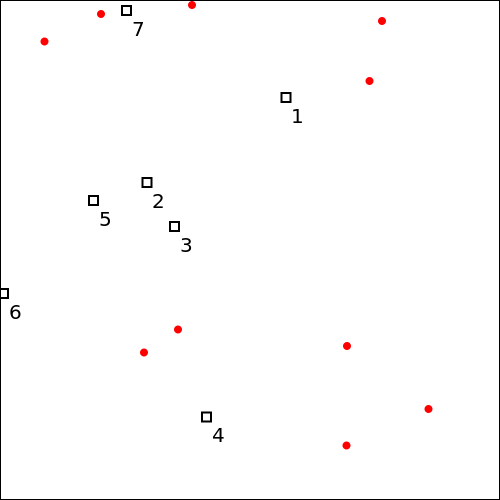
\includegraphics[width=5cm,height=5cm]{tiny_case_raw.png}}}
    \qquad \qquad \qquad
    \subfloat[Mejor solución encontrada con \texttt{POOL\_SIZE}$=5$.]{{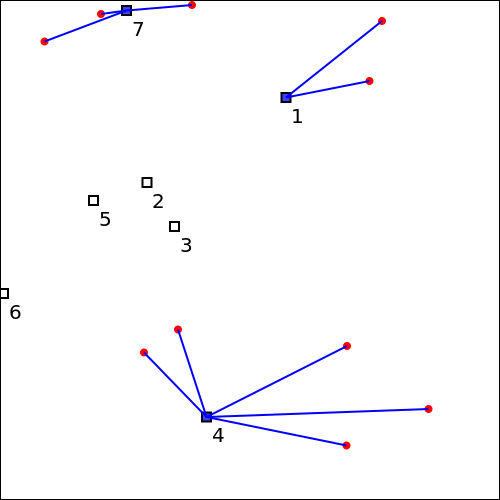
\includegraphics[width=5cm,height=5cm]{tiny_case_sol.png}}}
    \label{fig:ilustrative_problem}
\end{figure}

\begin{align*}
Z &= \{z_1,z_2,z_3,z_4,z_5,z_6,z_7\} \\
G &= \{z_1,z_2,z_3,z_4,z_5,z_7\} \\
B_1 &= \{\{z_1\},\{z_2\},\{z_3\},\{z_4\},\{z_5\},\{z_7\}\} \\
P_1 &= \{\{z_1\},\{z_2\},\{z_4\},\{z_5\},\{z_7\}\} \\
B_2 &= \{\{z_1,z_2\},\{z_1,z_3\},\{z_1,z_4\},\{z_1,z_5\},\{z_1,z_7\},\{z_3,z_7\},\{z_4,z_7\}\} \\
P_2 &= \{\{z_1,z_3\},\{z_1,z_4\},\{z_1,z_7\},\{z_3,z_7\},\{z_4,z_7\}\} \\
B_3 &= \{\{z_1,z_3,z_7\},\{z_1,z_4,z_7\}\} \\
P_3 &= \{\{z_1,z_3,z_7\},\{z_1,z_4,z_7\}\} \\
B_4 &= \{\} \\
\text{Mejor} &= \argmax_{S \in \cup_{i} (P_i)}\Phi(S) = \{z_1,z_4,z_7\}
\end{align*}

En primer lugar se calcula $G$, $z_6$ es excluído ya que $\{z_6\}$ no tiene valor positivo en la función objetivo y $G$ es también $B_1$.
En $P_1$ el proceso de reducción elimina $\{z_3\}$, producto de su similitud con $\{z_2\}$, logrando así obtener una \emph{pool} de tamaño $5$.
$B_2$ se construye agregando instalaciones de $G$ a las soluciones de $P_1$, nótese que, por ejemplo, la solución $\{z_2,z_7\}$ pudo haber sido generada en este proceso, tanto expandiendo $\{z_2\}$ con $z_7$ como expandiendo $\{z_7\}$ con $z_2$, pero no se agrega a la \emph{base} pues en la función objetivo no logró superar a alguna de estas soluciones que la pudo haber generado.
El proceso de reducción vuelve a eliminar soluciones parecidas hasta lograr $P_2$, al generar $B_3$ sólo resultan 2 soluciones pués el costo de agregar instalaciones sobrepasa la ganancia en la mayoría de estas. Para formar $P_3$ el proceso de reducció no hace nada pues hay menos de \texttt{POOL\_SIZE} soluciones, finalmente ninguna de las soluciones en $P_3$ puede expandirse de ninguna forma que genere una solución de tamaño 4 más rentable y la ejecución termina, entregando la mejor solución de entre todas las \emph{pools}.

\section{Reducción}

La idea principal del algoritmo, para prevenir la explosión combinatoria que sería explorar todas las posibles soluciones, es que, en cada iteración, la \emph{pool} contenga soluciones buenas pero \emph{representativas}. Para lograr esto, es necesario contar con una medida de disimilaridad entre las soluciones de la \emph{base}, e ir eliminando sistemáticamente soluciones que pueden ser representadas por otras similares, hasta que queden solo \texttt{POOL\_SIZE} de estas.

Si las soluciones fueran puntos en el espacio se podrían utilizar métodos de \emph{clustering} como \emph{k-means}, sin embargo, como son conjuntos de ubicaciones que tienen la misma cardinalidad no se puede utilizar estos métodos, por ejemplo, al unir dos soluciones en un mismo grupo, tener como representante del mismo grupo una posición promedio no es una opción.

Para realizar la reducción se requiere una medida de disimilaridad entre dos soluciones $A,B$ de la \emph{base} $B_n$ (y por lo tanto de tamaño $n$), llámese $D(A,B)$, siendo lógico que esta esté relacionada con la medida de distancia entre ubicaciones $d(u,v)$, las posibles medidas de disimilaridad se discutirán en la sección siguiente.

Un primer enfoque para resolver el problema de reducir las soluciones sería calcular las disimilaridades entre cada par de soluciones en la \emph{base}, encontrar el par con la menor dismilaridad y eliminar, de ambas, la que tenga el menor $\Phi$, repitiendo el proceso hasta que sólo quede la cantidad de soluciones requeridas.

El problema con esto es que una \emph{base} tiene $O(|X|$\texttt{POOL\_SIZE}$)$ soluciones y sería necesario calcular $O({|X|}^2$\texttt{POOL\_SIZE}$^2)$ disimilaridades, lo que también puede verse como $O({|Z|}^2$\texttt{POOL\_SIZE}$^2)$ si todas las ubicaciones de instalaciones son rentables.

Para evitar esto, dada la forma de la función objetivo y la medida de disimilitud, se puede asumir que si dos soluciones son similares \emph{geográficamente} (vale decír, respecto a que tan alejadas están sus ubicaciones de instalaciones) lo serán al ser evaluadas en la función $\Phi$. En
\ref{metricas_disimilitud} se explica la medida de disimilitud, en \ref{justificacion_reduccion} se justifica esta suposición.

En primer lugar, cada solución en la \emph{base} se ordena de mayor a menor valor tenga al ser evaluada en la función $\Phi$, luego, para cada una, se evalua su disimilitud sólo con las \texttt{VISION\_RANGE} siguientes, se detecta el par con la menor dismilaridad y del par se elimina el de menor $\Phi$. Tras esta eliminación, se calcula una disimilaridad más para cada una de las soluciones hasta \texttt{VISION\_RANGE} posiciones antes de la que se eliminó, a fin de que se sigan teniendo las disimilaridades \texttt{VISION\_RANGE} soluciones adelante. Este proceso se repite hasta que sólo quedan \texttt{POOL\_SIZE} soluciones.

Esta heurística puede ser aplicada para tener el mismo resultado que el primer enfoque, siempre y cuando \texttt{VISION\_RANGE} sea suficiente, porque se da que las soluciones más \emph{geograficamente} similares, tienen valor similares en la función $\Phi$ y, si no alcanzan a estar a lo mas a \texttt{VISION\_RANGE} posiciones en la \emph{base}, conforme esta se va reduciendo, lo estarán. Aplicar esto reduce la cantidad de disimilitudes a calcular de $O(|Z|^2$\texttt{POOL\_SIZE}$^2)$ a $O(|Z|$\texttt{POOL\_SIZE} \texttt{VISION\_RANGE}$)$.

\begin{figure}
\centering
\scriptsize

\subfloat[Detección de la disimilitud menor.]{
\begin{tabular}{ | c c c c c c c c c | }
\hline
$S_1$ & $S_2$ & $S_3$ & $S_4$ & $S_5$ & $S_6$ & $S_7$ & $S_8$ & $S_9$ \\
\hline
$D(S_1,S_2)$ & $D(S_2,S_3)$ & $D(S_3,S_4)$ & $D(S_4,S_5)$ & $D(S_5,S_6)$ &
$D(S_6,S_7)$ & $D(S_7,S_8)$ & $D(S_8,S_9)$ & \\
$D(S_1,S_3)$ & $D(S_2,S_4)$ & $\pmb{D(S_3,S_5)}$ & $D(S_4,S_6)$ & $D(S_5,S_7)$ &
 $D(S_6,S_8)$ & $D(S_7,S_9)$ & & \\
$D(S_1,S_4)$ & $D(S_2,S_5)$ & $D(S_3,S_6)$ & $D(S_4,S_7)$ & $D(S_5,S_8)$ &
$D(S_6,S_9)$ & & & \\
\hline
\end{tabular}
} \vfill

\subfloat[Eliminación de la solución de menor ganancia del par.]{
\begin{tabular}{ | c c c c c c c c c | }
\hline
$S_1$ & $S_2$ & $S_3$ & $S_4$ & \st{$S_5$} & $S_6$ & $S_7$ & $S_8$ & $S_9$ \\
\hline
$D(S_1,S_2)$ & $D(S_2,S_3)$ & $D(S_3,S_4)$ & \st{$D(S_4,S_5)$} & \st{$D(S_5,S_6)$} & $D(S_6,S_7)$ & $D(S_7,S_8)$ & $D(S_8,S_9)$ & \\
$D(S_1,S_3)$ & $D(S_2,S_4)$ & \st{$D(S_3,S_5)$} & $D(S_4,S_6)$ & \st{$D(S_5,S_7)$} & $D(S_6,S_8)$ & $D(S_7,S_9)$ & & \\
$D(S_1,S_4)$ & \st{$D(S_2,S_5)$} & $D(S_3,S_6)$ & $D(S_4,S_7)$ & \st{$D(S_5,S_8)$} & $D(S_6,S_9)$ & & & \\
\hline
\end{tabular}
} \vfill

\subfloat[Inserción de nuevas disimilitudes.]{
\begin{tabular}{ | c c c c c c c c c | }
\hline
$S_1$ & $S_2$ & $S_3$ & $S_4$ & \st{$S_5$} & $S_6$ & $S_7$ & $S_8$ & $S_9$ \\
\hline
$D(S_1,S_2)$ & $D(S_2,S_3)$ & $D(S_3,S_4)$ & \st{$D(S_4,S_5)$} & \st{$D(S_5,S_6)$} & $D(S_6,S_7)$ & $D(S_7,S_8)$ & $D(S_8,S_9)$ & \\
$D(S_1,S_3)$ & $D(S_2,S_4)$ & \st{$D(S_3,S_5)$} & $D(S_4,S_6)$ & \st{$D(S_5,S_7)$} & $D(S_6,S_8)$ & $D(S_7,S_9)$ & & \\
$D(S_1,S_4)$ & \st{$D(S_2,S_5)$} & $D(S_3,S_6)$ & $D(S_4,S_7)$ & \st{$D(S_5,S_8)$} & $D(S_6,S_9)$ & & & \\
 & $\pmb{D(S_2,S_6)}$ & $\pmb{D(S_3,S_7)}$ & $\pmb{D(S_4,S_8)}$ & & & & & \\
\hline
\end{tabular}
}
\caption{Ejemplo de un paso del proceso de reducción, se tienen 9 soluciones $S_1,S_2,...,S_9$ de mayor a menor función objetivo, inicialmente se tiene la disimilitud entre cada solución y las \texttt{VISION\_RANGE} siguientes (en este caso \texttt{VISION\_RANGE}$=3$). Una vez se encuentra la menor disimilitud se elimina la solución de menor función objetivo del par.\\ Finalmente se computan nuevas disimilitudes para que la disimilitudes de cada solución con sus \texttt{VISION\_RANGE} siguientes se sigan teniendo. El proceso se repite hasta que sólo quedan \texttt{POOL\_SIZE} soluciones.}
\label{fig:reduction}
\end{figure}


\section{Métricas de disimilitud}
\label{metricas_disimilitud}

Como se señaló previamente, para comparar soluciones se requiere una medida de disimilitud, siendo lógico que esté asociada a la métrica de distancia $d(a,b)$ entre dos ubicaciones $a,b$. Para que una medida $D(A,B)$ entre dos soluciones, $A = \{a_1,a_2,...,a_n\}$ y $B = \{b_1,b_2,...,b_m\}$, sea una métrica debe cumplir con:

\begin{enumerate}
\item $D(A,B) = 0 \Leftrightarrow A=B$
\item $D(A,B) = D(B,A)$
\item $D(A,C) \leq D(A,B) + D(B,C)$
\end{enumerate}

Para los experimentos se utilizará el \emph{mean geometric error} por su facilidad de cálculo. Esta métrica corresponde a la distancia promedio que tienen las ubicaciones de ambos conjuntos a la ubicación más cercana en el conjunto opuesto.

\begin{equation}
D(A,B) = \frac{1}{|A|+|B|}\left(\sum_{a \in A}\inf_{b \in B}d(a,b) +
\sum_{b \in B}\inf_{a \in A}d(b,a)\right)
\end{equation}

También se sugiere el \emph{minimum weight matching}. Esta métrica corresponde a la suma de las distancias entre los pares del matching completo $m^\star$ entre $A$ y $B$ que minimiza esta suma de distancias. $m^\star$ es, por lo tanto, la solución a un problema de asignación.

\begin{equation}
D(A,B) = \inf_{m \in M}\left( \sum_{(a,b) \in m} d(a,b)\right)
\end{equation}
Donde $M$ es el conjunto de todos los posibles matchings completos entre $A$ y $B$.

La razón de la elección de estas métricas es que consideran todos los elementos, haciendo que cualquier diferencia entre combinaciones de posibles ubicaciones sea considerada en el algoritmo. Si se utilizada, por ejemplo, \emph{simple linkage} o \emph{complete linkage} que sólo dependen del par de ubicaciones más cercano o más alejado respectivamente, sería común que dos soluciones, pudiendo ser bastante diferentes, tengan la misma disimilitud a una tercera, produciendo empates que se rompen arbitrariamente en el proceso de reducción.

\section{Experimentos y resultados}

\section{Conclusiones}

\bibliographystyle{amsplain}
\bibliography{main}{}

\end{document}
